\documentclass[a4paper,twoside,phd]{BYUPhys}
% The BYUPhys class is for producing theses and dissertations
% in the BYU Department of Physics and Astronomy.  You can supply
% the following optional arguments in the square brackets to
% specify the thesis type:
%
%   senior  : Produces the senior thesis preliminary pages (default)
%   honors  : Produces the honors thesis preliminary pages
%   masters : Produces the masters thesis preliminary pages
%   phd     : Produces the PhD dissertation preliminary pages
%
% The default format is appropriate for printing, with blank pages
% inserted after the preliminary pages in twoside mode so you can
% send it directly to a two-sided printer. However, for ETD
% submission the blank pages need to be removed from the final output.
% The following option does this for you:
%
%   etd     : Produces a copy with no blank pages in the preliminary section.
%             Remove this option to produce a version with blank pages inserted
%             for easy double sided printing.
%
% The rest of the class options are the same as the regular book class.
% A few to remember:
%
%   oneside : Produces single sided print layout (recommended for theses less than 50 pages)
%   twoside : Produces double sided print layout (the default if you remove oneside)
%
% The BYUPhys class provides the following macros:
%
%   \makepreliminarypages : Makes the preliminary pages
%   \clearemptydoublepage : same as \cleardoublepage but doesn't put page numbers
%                           on blank intervening pages
%   \singlespace          : switch to single spaced lines
%   \doublespace          : switch to double spaced lines
%
% --------------------------- Load Packages ---------------------------------

% The graphicx package allows the inclusion of figures.  Plain LaTeX and
% pdfLaTeX handle graphics differently. The following code checks which one
% you are compiling with, and switches the graphicx package options accordingly.
\usepackage{ifpdf}
\ifpdf
  \usepackage[pdftex]{graphicx}
\else
  \usepackage[dvips]{graphicx}
\fi

%%%%%%%%%%%%%%%%%%%%%%%%%%%%%%%%%%%%%%%%%%%%%%%%%%%%%%%%%%%%%%%%%%
% Edited : Beeshanga
%
% If you need to include any code in the text use this package
% \usepackage{listings}
% It can be used to make key words bold, add colours, etc. Refer
% to http://en.wikibooks.org/wiki/LaTeX/Packages/Listings for
% more information.
%
% For theorems, propositions, proofs and assumtions use this
% package
% \usepackage{amsthm}
% For more information refer to the following website
% http://en.wikibooks.org/wiki/LaTeX/Theorems
%
%%%%%%%%%%%%%%%%%%%%%%%%%%%%%%%%%%%%%%%%%%%%%%%%%%%%%%%%%%%%%%%%%%

% The fancyhdr package allows you to easily customize the page header.
% The settings below produce a nice, well separated header.
\usepackage{fancyhdr}
  \fancyhead{}
  \fancyhead[LO]{\slshape \rightmark}
  \fancyhead[RO,LE]{\textbf{\thepage}}
  \fancyhead[RE]{\slshape \leftmark}
  \fancyfoot{}
  \pagestyle{fancy}
  \renewcommand{\chaptermark}[1]{\markboth{\chaptername \ \thechapter. #1}{}}
  \renewcommand{\sectionmark}[1]{\markright{\thesection \ #1}}


% The cite package cleans up the way citations are handled.  For example, it
% changes the citation [1,2,3,6,7,8,9,10,11] into [1-3,6-11].  If your advisor
% wants superscript citations, use the overcite package instead of the cite package.
\usepackage{cite}

% The makeidx package makes your index for you.  To make an index entry,
% go to the place in the book that should be referenced and type
%  \index{key}
% An index entry labeled "key" (or whatever you type) will then
% be included and point to the correct page.
%\usepackage{makeidx}
%\makeindex

% The url package allows for the nice typesetting of URLs.  Since URLs are often
% long with no spaces, they mess up line wrapping.  The command \url{http://www.physics.byu.edu}
% allows LaTeX to break the url across lines at appropriate places: e.g. http://www.
% physics.byu.edu.  This is helpful if you reference web pages.
\usepackage{url}
\urlstyle{rm}

% If you have a lot of equations, you might be interested in the amstex package.
% It defines a number of environments and macros that are helpful for mathematics.
% We don't do much math in this example, so we haven't used amstex here.
\usepackage{amsmath}
\usepackage{amssymb}
\usepackage{subfigure}
\usepackage{cite}
\usepackage{amsxtra}
\usepackage{amsfonts}
\usepackage{graphicx}
\usepackage{multirow} % This is package for multi-rows in tables added on 7th July 2009 by Arif
%\usepackage{setspace}

% The caption package allows us to change the formatting of figure captions.
% The commands here change to the suggested caption format: single spaced and a bold tag
\usepackage[labelfont=bf,labelsep=colon]{caption}%[2008/04/01]
 \DeclareCaptionFormat{suggested}{\singlespace#1#2#3\par\doublespace}
 \captionsetup{format=suggested}


\usepackage{array}
\usepackage{multirow}
\usepackage{verbatim}
\usepackage{enumerate}

% Defining the symbols




% The hyperref package provides automatic linking and bookmarking for the table
% of contents, index, equation references, and figure references.  It must be
% included for the BYU Physics class to make a properly functioning electronic
% thesis.  It should be the last package loaded if possible.
%
% To include a link in your pdf use \href{URL}{Text to be displayed}.  If your
% display text is the URL, you probably should use the \url{} command discussed
% above.
%
% To add a bookmark in the pdf you can use \pdfbookmark.  You can look up its usage
% in the hyperref package documentation
\usepackage[bookmarksnumbered,pdfpagelabels=true,plainpages=false,colorlinks=true,
            linkcolor=black,citecolor=red,urlcolor=blue]{hyperref}

% ------------------------- Fill in these fields for the preliminary pages ----------------------------
%
% For Senior and honors this is the year and month that you submit the thesis
% For Masters and PhD, this is your graduation date
  \Year{2018}
  \Month{November 09,}
  \Author{Abhishek Satpathy}

% If you have a long title, split it between two lines. The \TitleBottom field defines the second line
% A two line title should be an "inverted pyramid" with the top line longer than the bottom.
    \TitleTop{Protocol for Smart Contract Communication}
  \TitleBottom{Among Blockchains} % edited Beeshanga
 \DegreeTitle{Bachelor of Engineering
 \\ Software Engineering Stream} % edited Beeshanga

% Your research advisor
 \Advisor{Supervisor: Michael Johnson}

% The department undergraduate research coordinator
%  \UgradCoord{A}

% The representative of the department who will approve your thesis (usually the chair)
%  \DepRep{B}

% Acknowledge those who helped and supported you

  \Acknowledgments{
  \vspace{-1.5cm}
    \noindent I would like to acknowledge my supervisor Prof. Michael Johnson who has always been a great help throughout my degree and not just this thesis. Michael accepted to supervise my project proposal even though it was not related to one of his areas of research. 
    
    
    \noindent I would also like to acknowledge Mr. Kris Crnomarkovic who has been really helpful with long and tiring discussions about certain difficult issues that I encountered during research. Kris's involvement with my theses is really appreciated.

  }


% The title of the department representative
%  \DepRepTitle{Chair}
  \Statement{
    \noindent I, Abhishek Satpathy, declare that this report, submitted as part of the requirement for the award of Bachelor of Engineering in the School of Engineering, Macquarie University, is entirely my own work unless otherwise referenced or acknowledged. This document has not been submitted for qualification or assessment at any other academic institution.
    \vspace{0.5cm}

    \noindent     Student's Name: Abhishek Satpathy

    \vspace{0.25cm}

    \noindent Student's Signature: Abhishek Satpathy

    \vspace{0.25cm}

    \noindent     Date: \today
    }

% The text of your abstract
\Abstract{
\vspace{-1.5 cm}
Blockchain technology has potential applicability in finance, supply-chain management, asset-tracking, web decentralization. Scalability and interoperbility are two major problems, hindering the applicability of blockchains in large-scale commercial architectures. Here, we discuss the application of a novel protocol that aims to solve the issues of scalability and interoperability of blockchains using a communication layer between multiple homogenous blockchains.
}



% Statement of Candidate



\fussy

\begin{document}

 % Start page counting in roman numerals
 \frontmatter

 %This command makes the formal preliminary pages.
 % You can comment it out during the drafting process if you want to save paper.

 \makepreliminarypages


%\clearemptydoublepage
\doublespace
%\include{Publications/publications}

% \clearemptydoublepage
%\include{Organization/organization}

 \clearemptydoublepage
\singlespace
 % Make the table of contents.
 \tableofcontents

\clearemptydoublepage
% Make the list of figures
\listoffigures

\clearemptydoublepage
% Make the list of tables
\listoftables

\clearemptydoublepage

% Start regular page counting at page 1
\mainmatter
%
\chapter{Introduction}
\label{chap:Introduction}
Blockchain technology has demonstrated enormous potential utility in multiple fields including "Internet of things", governance, finance, asset-tracking and web decentralization. However, the adoption and use of blockchains into production grade systems is yet to be demonstrated. 
 Scalability and inter-operability are major problems, hindering the production grade adoption of blockchains into these different fields of application. Blockchain systems currently are crippled by extremely low transaction  throughput which makes their use impractical in real world use cases. Available blockchain implementations are practically limited to around 30 transactions per second. This issue of limited transaction throughput arises from the current synchronous consensus mechanisms which require a wide time margin to ensure safety of the transactions. The demand for higher transaction throughput is rapidly increasing with the growing user base. One of the  ways of addressing this scalability problem is facilitating intercommunication among smart contracts on multiple separate blockchains. This intercommunication protocol inherently solves the problem of inter-operability along with scalability. In this thesis we lay out the design and implementations specifications of such a protocol that facilitates the inter-operability of multiple compatible blockchains.

\section{Project Goal}
The goal of this project is to lay out the design, implementation and testing specifications of a layer two blockchain solution that facilitates high transaction throughput and inter-operability among multiple blockchain systems. Layer two, here, is defined as a system that is built on top of a layer one blockchain system like ethereum or bitcoin and therefore relies on the layer one chain for security. Layer two solutions are built without requiring any breakthrough modifications to the existing layer one architecture. The project is specifically going to focus on a protocol that is built on top of ethereum as the foundation layer one blockchain. The biggest challenge for the implementation of this project is ensuring that the layer two solution is at least as secure as the existing foundation that it is built upon. The protocol has to balance between keeping a high transaction throughput and maintaining a high level of decentralization. Decentralization and transaction throughput can easily get inversely intertwined in a decentralized system architecture and therefore precaution needs to be taken while designing the system to reduce centralization.
\\
\\ One of the other goals of the project will also be to lay out the modifications to the existing foundation system that would allow the integration of the layer two system to the foundation architecture. The project does not aim to create a completely new blockchain architecture.
\section{Project Planning}
The project planning was done over the last six months during the course of ENGG 460. There have been a lot of changes the initial plan that was developed during ENGG 460. The biggest change however has been to the scope, deliverables and timeline of the project. These changes are discussed below in their respective sections.

\subsection{Scope}
The project scope has remained very similar to the scope that was described in the initial project plan. The scope is to deliver a protocol for intercommunication and interoperability of smart contracts. The scope in the initial project plan might have indicated that the scope includes the delivery of a prototype of such a blockchain architecture; however, the new scope of the project includes only the system requirements, design and testing specifications of the protocol. 
\subsection{Deliverables}
In the initial plan the project had two deliverables. One of the deliverables for the project was a suite of smart contracts on different ethereum blockchains such that those smart contracts can send messages and transactions among themselves. The other deliverable in the initial protect plan was a react-native app that would be able to demonstrate the functionality of the smart contracts. There has been a change in the deliverables for the project over the course of the last six weeks of progressing through the development. 
\\

The new deliverable for the project is a protocol for intercommunication and the interoperability of multiple blockchains. The deliverable includes system requirements, system design and testing specifications. However, any working prototype of the protocol is not a hard deliverable of the project.
\subsection{Timeline}
There have been significant changes to the timeline of the project as it has progressed over the last six weeks. The reason for these changes is the change in the deliverables for the project. The deadline for the project was assumed to mid December in the previous project plan; the new deadline is 9th of November which is a hard deadline. Moreover, a lot of variables and deliverables had unknown components with estimated timeframes. The timeline has a become firmer with most of the variables becoming clearer. The new GANTT chart with the updated timeline for the project is shown below.
\section{Project Background}
Prior to starting in on blockchain systems, one needs to be familiar with supporting technologies that support and facilitate the working of blockchains. 
\subsection{Cryptographic Hash Function}
A cryptographic hash function is a one way mathematical construct that takes a data input of arbitrary length and outputs arbitrary data of a fixed length. The primary use of hashing in cryptography is maintaining the integrity of messages. Hashes are used in a blockchain to ensure the integrity of the data stored in each block. The data or the list of transactions in a block is hashed and the hash is appended to the next block, this ensures the integrity of the data because if even a single bit of the data is manipulated then the new hash of the block is completely different. The hash function used in the protocol described in this paper is Keccac-512 which is a variation of the SHA-512 hashing algorithm. 
\subsection{Public Key Cryptography}
Public Key Cryptography is one of the core technologies used in a blockchain system. The accounts on a blockchain are a hashed version of the public key of the user. The accounts can be accessed 
\subsection{Consensus}
Consensus is a mechanism which ensures that every node on the blockchain network has the same exact copy of the data. A consensus mechanism syncs data across all nodes as and when those nodes connect to the network. Consensus also works as a fault tolerance mechanism which is essential in any distributed computing setup suck as a distributed ledger to avoid corrupt nodes. Proof of work is by far the most popular consensus mechanism used in mainstream public blockchains. It is a ultimately a variation of the popular Practical Byzantine Fault tolerance algorithm.
\subsection{State Transition Machine}
The state on a blockchain is a mapping between the account addresses and the state of the account in terms of the transaction history. Every transaction on the blockchain is a manupulation of the state. The blockchain itself acts as a state transition machine which facilitates transactions by allowing the valid ones to manipulate the state.
\subsection{Clients}
A client of the blockchain is the end-user software that ensures the blockchain synchronisation, generates and stores private keys, and facilitates transactions on behalf of the private key. Clients live on user hardware which act as an interface between the user's device and the blockchain network.
\subsection{Transactions}
A transaction is a the transfer of a signed data package on the blockchain which manipulates the state of the ledger. It is a record of a valid computational activity that has taken place. Any information that is stored and can be retrieved is the result of a transaction. EVM transactions involve transfer of value as the transaction themselves have a cost attached to them. 
\subsection{Smart Contracts}
Smart Contracts are agents that facilitate the negotiation of a transaction on the blockchain without the use of another third party agent. Smart contracts are the only entry point to the state of the blockchain and therefore the only party that can modify the data layer on the ledger.

\chapter{Background and Related Work}
Before any meaningful research is done on the topic, it is quite essential to review the available literature on the topic. The process of reviewing existing literature review helps one to understand the cutting edge research on the topic and also familiarize oneself with failures and successes. This chapter reviews the existing literature and work done in the area of increasing blockchain transaction throughput by facilitating interoperability of blockchains. The most important thing to note is that there is a serious lack of quality academic literature in the field as the research in the field is quite new and hasn't percolated into academia yet. Therefore, most of the available literature is from research work done by blockchain startups and the available whitepapers. The language in those whitepapers is often not very academic and therefore one of the most important tasks in this chapter would be to interpret the whitepapers critically and translate the language into proper academic form.
\section{Ethereum}
The entire framework of this project is based on the ethereum protocol. Therefore, the discussion on ethereum is unavoidable. Ethereum is a decentralised value transfer system made possible using a cryptographically secure, transaction-based state machine. A blockchain or a distributed ledger in simple terms. Ethereum was first developed by Vitalik Buterin in late november 2013. It was a complete rewrite of the bitcoin system with addition of a turing-complete virtual machine and smart contract execution capability. In ethereum's state transition machine, the final state also referred to as the canonical state is a result of a consensus mechanism using a simplified version of the GHOST protocol.

\subsection{Blocks, State and Transactions}
\subsubsection{Blocks}
The block in Ethereum is a collection of transaction bunched together as a set. The block has three parts, a block header, the transactions, and the ommers which is a collection of related block headers. The block header contains the following pieces of information:
\begin{description}
\item[$\bullet$ parentHash:] a Keccak 256-bit hash of the previous block's header
\item[$\bullet$ ommersHash:] a Keccak 256-bit hash of the ommers list or the list of blocks which have the same parent block as the current block
\item[$\bullet$ beneficiary:] the 160-bit address of the account to which all the gas fee has to be transferred
\item[$\bullet$ stateRoot:] a Keccak 256-bit hash of the root node of the state trie
\item[$\bullet$ transactionsRoot:] a Keccak 256-bit hash of the root node of the trie containing all the transactions in the current block
\item[$\bullet$ receiptsRoot:] a Keccak 256-bit hash of the trie containing the reciepts of all the transactions in the current block
\item[$\bullet$ logsBloom:] bloom filter composed of index-able log entries for transaction receipts
\item[$\bullet$ difficulty:] a number corresponding to the difficulty level of the block
\item[$\bullet$ number:] a scalar value corresponding to the number of ancestor blocks of the current block. The genesis block does not have an ancestor block and hence, it is conventionally assigned a number 0.
\item[$\bullet$ gasLimit:] a scalar value equal to the maximum limit of gas expenditure of the block
\item[$\bullet$ gasUsed:] a scalar value equal to the total gas used in transactions in the block
\item[$\bullet$ timeStamp:] a reasonable output of the Unix's time at the block's inception
\item[$\bullet$ extraData:] arbitrary byte array containing block metadata
\item[$\bullet$ mixhash:] a 256-bit hash which together with the nonce proves that a sufficient amount of computation has been carried out on this block
\item[$\bullet$ nonce:] a 64-bit hash which together with the mix-hash proves that a sufficient amount of computation has been done on this block
\end{description}
\subsubsection{World State}
The world state is a mapping between account addresses which are 160 bit hashed versions of the public keys and account states. This mapping is stored in a data-structure called a Merkle Patricia tree. The account states comprise of the following fields;
\begin{description}
\item[$\bullet$ nonce:] it is a value that is equal to the number of transactions sent from the account
\item[$\bullet$ balance:] a value equal to the number of wei owned by the address
\item[$\bullet$ storageRoot:] a 256-bit hash of the root node of the merkle patricia tree that contains the storage data of the account
\item[$\bullet$ codeHash:] the hash of the EVM code of the account, which gets executed in case of transactions
\end{description}
\subsubsection{Transactions}
A transaction is formally a single cryptographically signed instruction executed by an external party. There are two types of transactions in Ethereum: the first type results in a message call between actors and the second type results in creation of new accounts. A transaction primarily has the following fields:
\begin{description}
\item[$\bullet$ nonce:] a value equal to the number of transactions sent by the sender
\item[$\bullet$ gasPrice:] number of wei to be paid for each unit of gas. Gas is a computational unit in the EVM which is discussed in a later section.
\item[$\bullet$ gasLimit:] maximum amount of gas that should be utilised for executing this transaction
\item[$\bullet$ to:] a 160-bit address of the message call's recipient 
\item[$\bullet$ value:] number of wei to be transferred to the message call's recipient
\end{description}
A contract creation account contains the following additional fields:
\begin{description}
\item[$\bullet$ nonce:] infinite size byte array containing the EVM code for account initialisation
\item[$\bullet$ data:] infinite size byte array containing the input data of the message call
\end{description}
\begin{description}
\item[]
\end{description}
\subsection{Gas and Transaction Execution}
Gas and transactions are the core of the ethereum computation engine. Transactions forms the basis for all the computation and Gas forms the basis of all payment calculation in ethereum.
\subsubsection{Gas}
Gas is defined as any programmable computation in ethereum. The Ethereum Virtual Machine is a turing-complete computation engine and it is absolutely essential to limit the possibility of denial-of-service attacks in a public computation engine. Gas costs ether to execute and therefore prevents denial-of-service as no ethereum account is likely to have an infinite amount of ether. Every transaction has a gas price which is the amount of ether paid per gas or computational step. Miners will usually preferably select a transaction which has the highest gas price.
\subsubsection{Sub-state}
A valid transaction in ethereum is defined as a transaction which:
\begin{description}
\item [$\bullet$ is a well formed RLP;]
\item [$\bullet$ has a valid signature;]
\item [$\bullet$ has a valid nonce;]
\item [$\bullet$ has a gas limit which is not less than the intrinsic gas;]
\item [$\bullet$ has a sender whose account balance greater than the gas cost]
\end{description}

A transaction is also the most complex part of the ethereum virtual machine as it involves the state transition mechanism. The virtual machine gets in transition state during the execution of the transaction, called the substate. The substate creates a set of temporary accounts needed to complete the transaction, called the suicide set.

The ethereum state transition function is defined as follows:

\subsection{Canonicalisation}
\subsection{Message Call}
\section{Polkadot}
Polkadot is another approach by the ethereum community to solve the issue of scalability and interoperability by developing a multi-chain framework. Currently, Polkadot is far from being a working system or a prototype 
\section{Cosmos}
Cosmos is a platform which facilitates the interoperability of multiple parallel blockchains while retaining the inherent security features of blockchains. One of the problems faced by interoperable multi-chain frameworks is their vulnerability to an attack if a majority of the hashing ability is not merge-mined with the central parent chain. Cosmos addresses this issue by having multiple independent blockchain which are called zones in Cosmos. The central or the parent chain is called the Cosmos hub. The zones utilise something called a Tendermint Core, which is a Practical Byzantine Fault Tolerant consensus engine. The system described in this paper uses Tendermint and it will be discussed in a later section.

The main currency on the Cosmos hub is a multi-asset proof-of-stake token. The hub and zones facilitate the intercommunication between the hub and the zones using a protocol called the interblockchain comunication protocol, which works on a virtual UDP layer for blockchains.

\subsection{Consensus}
Cosmos uses a partially synchronous BFT (Byzantine Fault Tolerant) consensus algorithm called Tendermint. It uses optimal Byzantine Fault Tolerance with a super majority of greater than 2/3 of the total voting power. Hence, greater than a third of the total voting power has to be Byzantine to cause a violation of safety. In case, a violation occurs, it can be detected by the system by detecting conflicting blocks. And since Cosmos combined with Tendermint is a permissioned system, it is much easier to detect Byzantine nodes.

\subsection{The Hub and Zones}
The Hub and different zones in Cosmos are connected using a protocol called Interblockchain-communication (IBC) protocol. The block commits in the zones are are constantly posted on the hub, allowing the hub to keep track of the world state and also the state of the zones. The zones communicate among each other using the IBC protocol, by sending Merkle-proofs of transactions. 
\subsubsection{The Hub}
The Cosmos hub is the central blockchain in the system which hosts a distributed ledger that supports multiple tokens. These coins are moved from one zone to another using a speacial packet in IBC called a coin packet. The hub is accountable for counting the total amount of coins in each hub. The hub is the central ledger responsible for the entire network of the zones and therefore, is a single point of failure. The security of the hub is of paramount importance. It is secured by a global set of validators which are all permissioned nodes.
\subsubsection{The Zones}
The Zones exchange information among each other via the hub using the IBC. A zone is a essentially a multi-asset, multi-signature account. The hub ensures that the zones cannot transfer more tokens than it has been assigned. The hub does not verify the authenticity of the zones and therefore it should within the senders' discretion to send tokens across zones. 
\subsection{Inter-blockchain Communication (IBC)}
The Inter-blockchain communication (IBC) works by moving packets of data from one zone to another via the hub by posting Merkle-proofs. The proof is evidence that the sending chain published a packet which was meant for the receiving chain. 

The IBC is the most important component of the Cosmos literature. IBC is mentioned here because a lot of inspiration for communication between different blockchains, which have been mentioned in later chapters actually come from the IBC protocol. As shown in the diagram below, the IBC has two different types of transactions; namely, IBCBlockCommitTx transaction and an IBCPacketTx transaction. The IBCBlockCommitTx allows a zone to prove to any observer zone that its most recent block hash exists. The IBCPacketTx allows a zone to prove to any observer that a published packet was indeed sent by the sender. The separation of the two different types of transactions allows the sender and receiver zones to have independent control over their block commits, respectively. The IBCBlockCommit interaction diagram which shows the two types of transactions has been shown in figure 2.1 above.
\begin{figure}
  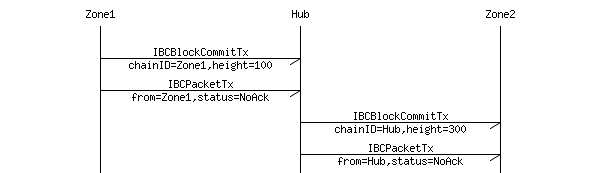
\includegraphics[width=\linewidth]{ibc_transactions.png}
  \caption{IBCBlockCommit Transaction interaction diagram.}
  \label{fig:1}
\end{figure}

\section{Zilliqa}
Zilliqa is another blockchain solution which aims to solve the problem of scalability by using blockchain sharding. It divides the mining network into smaller shards, each capable of processing transactions in parallel. It also has a smart contract execution environment or a virtual machine and a special contract language which implements data-flow programming. This allows the parallel processing of the programs as soon as all the inputs are available. The entire system in Zilliqa is divided into six layers. This layering system is good for maintenance and abstraction of different parts of the system. The layers are explained in more detail in the sections below:

\subsection{Cryptographic Layer}
Zilliqa's cryptographic layer uses elliptic curve cryptography for digital signatures and a memory hard hash function for proof-of-work (PoW). The hash function used in Ziliqa is ethash, which is the hash function used in ethereum. Ethhash is based on Keccak, which is memory hard meaning that Application specific integrated circuits (ASIC) will not be able to generate the hashes. 
\subsubsection{EC-Schnorr Signature}
Zilliqa uses digital signatures based on the EC-Schnorr algorithm instantiated with the secp256k1 elliptic curve. According to Zilliqa, EC-Schnorr has a few benefits over Elliptic Curve Digital Signature Algorithm (ECDSA). Those benefits are Non-malleability, Multisignature ability, and faster speeds. 

\subsubsection{Proof of Work}
Zilliqa uses Proof of Work to prevent Sybil attacks and generate node identities. This is contrary to other blockchain systems such as Ethereum which use PoW for the purpose of achieving consensus. Sybil attacks work by forging identitites of different systems in order to subvert the reputation of the concerned system, especially in used in peer-to-peer networks. Zilliqa uses ethhash as its algorithm of choice for PoW. As mentioned earlier, ethash is a memory hard hash function and requires a considerable amount of memory and high bandwidth I/O interface which makes it impossible to use specialised hardware for computation of the hash.
\subsection{Data Layer}
The data layer mainly consists of the global state of Zilliqa and it also defines the data needed by different entities to update the global state. 
\subsubsection{Accounts and Addresses}
Zilliqa just like ethereum is an account based blockchain system and consists of two types of accounts; namely, a normal account and a contract account. A normal account is created when the EC-Schnorr algorithm is invoked to create a private key. A contract account is created when a contract is deployed by another normal account. The public key is then derived from the private key by using the EC-Schnorr algorithm. The account address for a normal account is then generated by using the 160 least significant bits of the SHA-3 hash of the public key and for a contract account it is generated by using the 160 least significant bits of the SHA-3 hash of the address of the creator's account and the account nonce, which is the number of transactions sent from the particular account. The equations for generating the addresses for both normal and contract accounts are given below:
\begin{equation}
    A_{normal} = LSB_{160}(SHA3-256(PubKey(sk)))
\end{equation}
\begin{equation}
    A_{contract} = LSB_{160}(SHA3-256(address||nonce))
\end{equation}

Each account is associated with an account an account state which has the following information:
\begin{description}
\item[$\bullet$ account nonce:] the number of transactions sent from the account in case of a normal account, or the number of transactions sent from the creator's account in case of a contract account.
\end{description}
\subsection{Network Layer}
\subsection{Consensus Layer}
\subsection{Smart Contract Layer}
\subsection{Incentive Layer}

\section{Tendermint}

\label{chap:LitReview}

\chapter{System Requirements}
\label{chap:singleuser}

\section{System Overview \label{sec:Intro-ChapUserSelec}}

\section{System Features \label{sect:chap2sysmodel}}

\section{Other Non-Functional Requirements}

\chapter{System Specifications and Design}
\label{chap:Conclusions}
\chapter{System Implementation}
\chapter{Discussion}
\chapter{Conclusions}
\chapter{Future Work}
\chapter{Abbreviations}
\label{chap:abbreviations}

\begin{tabbing}

AWGN \qquad \qquad \= Additive White Gaussian Noise\\
BC \> Broadcast Channel\\
BS \> Base Station\\
CSI \> Channel State Information\\
CSIR \> Channel State Information at Receiver\\
CSIT \> Channel State Information at Transmitter\\
dB \> Decibels\\
DPC \> Dirty Paper Coding\\
GS \> Gram-Schmidt\\
RVQ \> Random Vector Quantisation\\
SISO \> Single Input Single Output\\
SNR \> Signal to Noise Ratio\\
SINR \> Signal to Interference plus Noise Ratio\\
MISO \> Multiple Input Single Output\\
SIMO \> Single Input Multiple Output\\
MIMO \> Multiple Input Multiple Output\\
MMSE \> Minimum Mean Square Error\\
MRC \> Maximum Ratio Combining\\ 
QoS \> Quality of Service\\
TDD \> Time Division Duplex\\
FDD \> Frequency Division Duplex\\
ZF \> Zero-Forcing\\
ZFBF \> Zero-Forcing Beamforming\\
ZMCSCG \> Zero Mean Circularly Symmetric Complex Gaussian\\

\end{tabbing}

%\phantomsection \addcontentsline{toc}{chapter}{Index}
% \renewcommand{\baselinestretch}{1} \small \normalsize
% \printindex

\appendix
\chapter{name of appendix A}
\section{Overview}
here is the Overview of appendix A ...
\section{Name of this section}
here is the content of this section ...
\chapter{name of appendix B}
\section{Overview}
here is the Overview of appendix B ...
\section{Name of this section}
here is the content of this section ...

%\input{Bibliography/biblio3}
\bibliographystyle{IEEEtranS}
%\bibliographystyle{acm}
\bibliography{my_reference}
%\bibliography{Bibliography/biblio4}


\end{document}
